%%  hyp_a = 0.8 # x-intercept of hyperbola
%%  hyp_c = 1.2 # x-value of hyperbola focal point
%%  
%%  ell_b = 1.5 # length of short radius for ellipse
%%  ell_c = 2.1 # distance between center and focal point for ellipse
%%  ell_th = 0.5 # theta rotation angle (radians) of ellipse (ccw)
%%  ell_a = sqrt(ell_b^2 + ell_c^2)
%%  
%%  # want the left focal point of the ellipse to match the left focal point of the hyperbola:
%%  ell_x = ell_c*cos(ell_th) - hyp_c # ellipse center x
%%  ell_y = ell_c*sin(ell_th) # ellipse center y
%%  
%%  ell_rfx = ell_x + ell_c*cos(ell_th) # ellipse right focal point x
%%  ell_rfy = ell_y + ell_c*sin(ell_th) # ellipse right focal point y
%%  ell_lfx = ell_x - ell_c*cos(ell_th) # ellipse left focal point x
%%  ell_lfy = ell_y - ell_c*sin(ell_th) # ellipse left focal point y
%%  
%%  var('x y')
%%  xmin = -2.5
%%  xmax = 3.5
%%  ymin = -1.5
%%  ymax = 3.5
%%  
%%  hyp = (x^2)/(hyp_a^2) - (y^2)/(hyp_c^2 - hyp_a^2) == 1
%%  hyp_plot = implicit_plot(hyp, (x, xmin, xmax), (y, ymin, ymax), color="red")
%%  
%%  ell = (((x - ell_x)*cos(ell_th) + (y - ell_y)*sin(ell_th))^2)/(ell_a^2) + (((x - ell_x)*sin(ell_th) - (y - ell_y)*cos(ell_th))^2)/(ell_b^2) == 1
%%  ell_plot = implicit_plot(ell, (x, xmin, xmax), (y, ymin, ymax))
%%  
%%  g = Graphics()
%%  g += hyp_plot
%%  g += ell_plot
%%  g += point((-hyp_c, 0), size=35, color="red", alpha=0.5)
%%  g += point((hyp_c, 0), size=35, color="red", alpha=0.5)
%%  g += point((ell_x, ell_y), size=35, alpha=0.5)
%%  g += point((ell_rfx, ell_rfy), size=35, alpha=0.5)
%%  g += point((ell_lfx, ell_lfy), size=35, alpha=0.5)
%%  g.show()

\section{Optics - Mirrors}

In this lab you will study the reflective properties of curved mirrors.

\hfill \break
\underline{Part 1 - Hyperbolic Mirrors}
\hfill \break

Consider the hyperbola
%
\begin{equation}
\label{eq:hyperbolaEq}
\frac{x^2}{0.8^2} - \frac{y^2}{1.2^2 - 0.8^2} = 1
\end{equation}
%
shown if figure~\ref{fig:hyperbolaPlot}.
Choose a light ray originating from the right-most region of the plot and heading towards the left focal point.
Show mathematically that when this ray is reflected by the hyperbolic mirror, it will pass through the second focal point.
Use a ruler to \textit{accurately} draw the path of this ray, stopping at the second focal point.
Draw the path for at least two more rays that are also initially headed towards the left focal point.
%
\begin{figure}[!h]
\centering
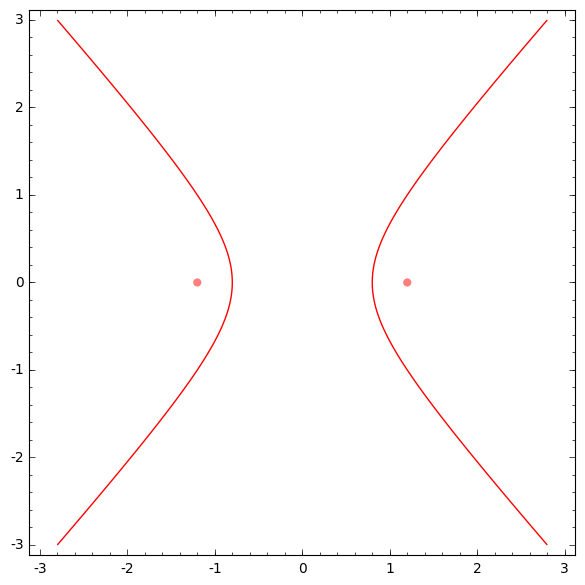
\includegraphics[scale=0.85]{figures/optics-mirrors/hyperbolaPlot.png}
\caption{The hyperbola defined in equation~\ref{eq:hyperbolaEq}.}
\label{fig:hyperbolaPlot}
\end{figure}

%%%%%%%%%%%%%%%%%%%%%%%%%%%%%%%%%%%%
%%%%%%%%%%%%%%%%%%%%%%%%%%%%%%%%%%%%

\hfill \break
\underline{Part 2 - Elliptical Mirrors}
\hfill \break

Consider the ellipse
%
\begin{equation}
\label{eq:ellipseEq}
\frac{x^2}{1.5^2 + 2.1^2} + \frac{y^2}{1.5^2} = 1
\end{equation}
%
shown if figure~\ref{fig:ellipsePlot}.
Choose a light ray originating from the right-most focal point.
Show mathematically that when this ray is reflected by the elliptical mirror, it will pass through the second focal point.
Use a ruler to accurately draw the path of this ray, stopping at the second focal point.
Draw the path for at least two more rays that also originate from the right-most focal point.
%
\begin{figure}[!h]
\centering
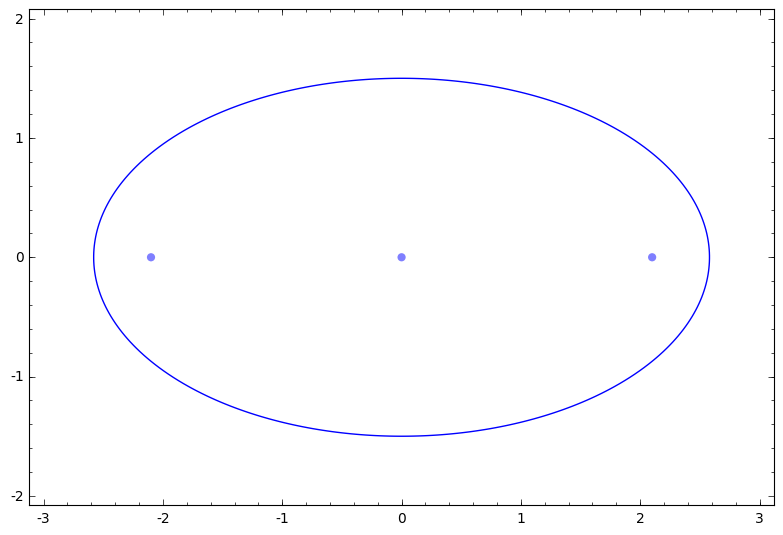
\includegraphics[scale=0.85]{figures/optics-mirrors/ellipsePlot.png}
\caption{The ellipse defined in equation~\ref{eq:ellipseEq}.}
\label{fig:ellipsePlot}
\end{figure}

%%%%%%%%%%%%%%%%%%%%%%%%%%%%%%%%%%%%
%%%%%%%%%%%%%%%%%%%%%%%%%%%%%%%%%%%%

\hfill \break
\underline{Part 3 - Mirror Combinations}
\hfill \break

As shown in figure~\ref{fig:both}, an ellipse and hyperbola share a focal point (left-most point).
Use a ruler, plus the rules of reflection from parts 1 and 2, to accurately draw the location where all\footnote{consider only rays that hit the ellipse first} rays originating from the right-most point intersect.
%
\begin{figure}[!h]
\centering
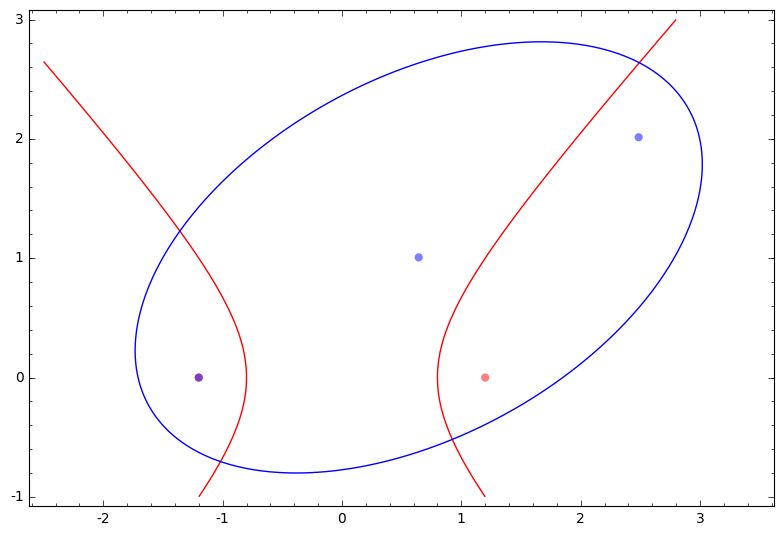
\includegraphics[scale=0.85]{figures/optics-mirrors/both.png}
\caption{An ellipse and a hyperbola sharing a focal point.}
\label{fig:both}
\end{figure}

\pagebreak \clearpage
